
\documentclass[12pt]{article}
\usepackage{fullpage}
\usepackage{graphicx}
\usepackage{indentfirst}
\usepackage{amsmath}


\begin{document}

\begin{titlepage}
\begin{center}

\setlength{\topskip}{3cm}
\center{\huge{\textsc{ -\\ }}}
\vspace{10 cm}

\includegraphics[scale=0.75, origin=c]{figures/PSU-logo.eps} \\
\vspace{0.75 cm} 
\large{Sahand Noorizadeh } \\
\vspace{0.25 cm} 
\large \today \\
\vspace{1.5 cm}
COURSE TITLE2
\end{center}
\end{titlepage}

\section{Problem Formulation}
\subsection{Understanding Phase Objects}

\begin{figure}[h]
	\centering
	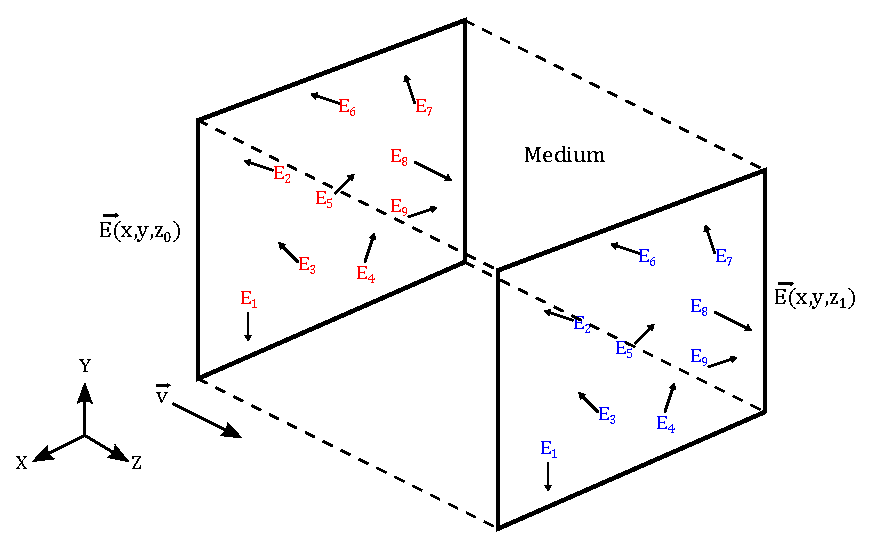
\includegraphics[scale=1]{figures/field_prop.eps}
\end{figure}

\begin{equation}
U(x,y,z) = A(x,y)\mathrm{e}^{-i\left[\,\omega \, t - \vec{k} \,\cdot \,\hat{n} \, d - \Phi(x,y)\,\right]} 
\end{equation}
For a thin phase object ($d<<1$) with negligible effect on the amplitude, the above expression becomes:
\begin{equation}
U(x,y,z) =\mathrm{e}^{-i\,\omega \, t} \, \mathrm{e}^{i\,\Phi(x,y)} 
\end{equation}

The input phase pattern is:
\begin{equation}
\Phi(x,y) = \cos(\psi_x \, x) + \cos(\psi_y \, y) 
\end{equation}


\end{document}
